Während sich agile Praktiken im Hinblick auf die Softwareentwicklung auf eine kontinuierliche Planung, Flexibilität und eine schnelle Reaktion auf sich ändernde Kundenanforderungen fokussieren, können DevOps-Praktiken dazu verwendet werden, den Arbeitsfluss vom Kunden über die Entwicklung, den Betrieb und zurück kontinuierlich auszubauen und damit die Qualität und Belastbarkeit der Software zu steigern \cite{fitzgerald_continuous_2014} \cite[S. 264]{tokarski_strategische_2018}. Die \textit{'Continuous Everything'}-Methoden spiegeln die Idee einer kontinuierlichen Verbesserung und Automatisierung innerhalb eines Devops-Prozesses wieder. Wie in Abbildung 2.7 zu erkennen ist, können sich diese Methoden auf mehrere Entwicklungsphasen konzentrieren und werden in diesem Abschnitt im Einzelnen beschrieben.  

\begin{figure}[h]
    \centering
    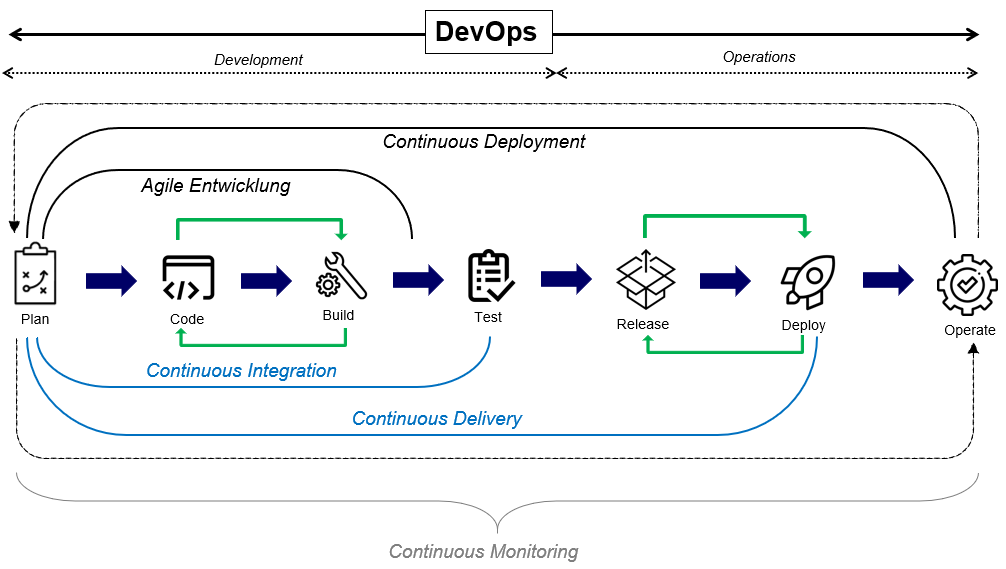
\includegraphics[scale=0.5]{Bilder/Continuous Everything.png}
    \caption{Continuous-Methoden innerhalb des Devops-Lebenszykluses, angelehnt an \cite[S. 16]{halstenberg_devops_2020}}
\end{figure}

\subsubsection{2.1.6.1. Agile Entwicklung} $~$

Die agile Entwicklung beschreibt die Verwendung von agilen Methoden innerhalb des Softwareentwicklungsprozesses als eine wesentliche Grundvoraussetzung für den DevOps-Prozess. Oftmals wird dieser Prozess auch als Continuous Planning (dt. kontinuierliches Planen) bezeichnet und reicht von der Phase des Planes bis zur Phase des Builds \cite{fitzgerald_continuous_2014}. Ziel ist es, sicherzustellen, dass die Investitionsentscheidungen während des gesamten Lebenszyklus auf die Bedürfnisse des Kunden abgestimmt worden sind. 

\subsubsection{2.1.6.2. Continuous Integration} $~$

Die Methode des Continous Integration (dt. kontinuierliche Integration, kurz: CI) beschreibt grundsätzlich die Gewährleistung einer sicheren und lückenlosen Integration von Codeänderungen in die vorhandenen Umgebungen \cite[S. 266]{tokarski_strategische_2018}. Ziel ist es, die Qualität der Software sicherzustellen und schnelles Feedback über die Integrierbarkeit vor der Auslieferung zum Kunden zu erhalten \cite[S. 266]{tokarski_strategische_2018}. Kernelement stellt ein Versionsverwaltungssystem (auch: Repository) dar, dessen wesentliche Aufgabe es ist, den DevOps-Teams dabei zu helfen, den Code von mehreren Entwicklern zu organisieren, Änderungen zu verfolgen und automatisierte Tests zu ermöglichen. Zunächst werden neuer oder geänderter Code nach der Entwicklung und Prüfung regelmäßig und in möglichst kurzen Abständen in einem gemeinsamen Repository gemergt (dt. zusammengeführt) \cite[S. 13-16]{sharma_devops_2017}. In diesem Zuge wird der Code automatisiert in einem Build kompiliert. Die neu erstellten Artefakte, werden in eine lauffähige Umgebung integriert und automatisiert getestet um sicherzustellen, ob die neuen Codeänderungen einer Komponente innerhalb der gesamten Anwendung lauffähig sind.\\\\ Dies ist essentziell für den Prozess, da häufig viele Entwickler an der Codebasis mit leicht unterschiedlichen Versionen arbeiten und daher überprüft werden muss, ob die verschiedenen Änderungen richtig zusammenarbeiten \cite[S. 69]{verona_practical_2016}. Aufgrund des regelmäßigen Integrierens der Codeänderungen wird gewährleistet, dass häufige automatisierte Tests durchführt werden, den Entwicklern stets der aktuellste Code zur Verfügung steht und Entwickler nicht darauf warten müssen, einzelne Codeabschnitte am Tag der Veröffentlichung auf einmal zu integrieren \cite{thedev_eight_2019}. Durch die entstehende Flexibilität und Geschwindigkeit können Fehler schneller und leichter behoben werden, da die Programmbestandteile kleiner und weniger komplex sind und das Debugging insgesamt sinkt \cite{thedev_eight_2019}. Wie an der Abbildung zu erkennen ist, umfassen die CI-Schritte die Codekompilierung, die Durchführung von Unit- und Akzeptanztests, die Validierung der Codeabdeckung, die Überprüfung der Einhaltung von Codierungsstandards und die Erstellung von Bereitstellungspaketen \cite{fitzgerald_continuous_2014}. 

\subsubsection{2.1.6.3. Continuous Delivery} $~$

Bei dem Ansatz des Continuous Delivery (dt. kontinuierliches Ausliefern, kurz: CD) handelt es sich um die nächste Stufe des Continuous Integration. Die Methode der Continuous Delivery baut auf einer regelmäßigen und automatisierten Bereitstellung des Builds an den Testbereich, zur anschließenden Bewertung und einer potentiellen Freigabe, auf \cite[S. 16 - 18]{sharma_devops_2017}. Da regelmässig Builds durch die Continuous Integration erzeugt werden, müssen diese zeitnah in andere Umgebungen weitergeleitet werden \cite[S. 16 - 18]{sharma_devops_2017}. Voraussetzung ist der Aufbau einer Continuous-Delivery-Pipeline, mit dem Ziel, das Ausliefern der Software möglichst automatisiert für die Bereitstellung neuer Releases durchzuführen \cite[S. 10]{wolff_continuous_2016}. \\\\ Sobald ein neues Artefakt innerhalb des Repositorys übertragen wurde, wird die Continuous-Delivery-Pipeline ausgelöst, wie in Abbildung 7 zu sehen ist \cite[S. 14]{verona_practical_2016}. In diesem Rahmen werden die fehlerfreien Builds automatisiert innerhalb eines produktionsähnlichen Staging- oder Testbereich bereitgestellt, um nach dem Testen zu bewerten, wie sich die neu entstandene Version des Builds produktionsnah verhält und letztlich in die Produktion verlagert werden kann \cite[S. 16]{sharma_devops_2017}, \cite{thedev_eight_2019}. Falls das Testen in der Pipeline fehlschlägt, werden die Entwickler informiert und haben die Gelegenheit, kurzfristig Anpassungen an dem jeweiligen Build vorzunehmen oder diesen zu verwerfen. Die Methode des Continuous Delivery beinhaltet mehrere Vorteile für das gesamte DevOps-Team. So wird aufgrund des hohen Grades an Automatisierung der Release-Prozess maßgeblich verbessert, indem Risiken und Engpässe durch die häufige Auslieferung von kleinen Features vermieden werden können und damit ein kontinuierlicher Integrationsfluss sichergestellt werden kann \cite[S. 18]{wolff_continuous_2016}.

\subsubsection{2.1.6.4. Continuous Deployment} $~$

Die letzte Phase der Delivery-Pipeline ist das Continuous Deployment (dt. kontinuierliche Bereitstellung, kurz: CD). Kernaufgabe des Continuous Deployments ist die voll automatisierte Überführung des Codes in die Produktivumgebung mithilfe der Delivery-Pipeline \cite[S. 29]{alt_innovationsorientiertes_2017}. Aufgrund der automatisierten Freigabe des Releases, muss sowohl die Qualität als auch die Lauffähigkeit der Pipeline besonders gesichert sein und ist daher abhängig von der Phase des Continuous Delivery \cite[S. 269]{tiemeyer_handbuch_2021}. Continuous Deployment entspricht der höchsten Stufe einer Delivery-Pipeline, was den DevOps-Teams ermöglicht, kleinste Features und Änderungen automatisiert für den Anwender ausliefern zu können. Dies wäre theoretisch das höchste Ziel der voll automatisierten Softwareentwicklung \cite{humble_why_2011}. Durch diesen höchsten Grad können die Vorlaufzeiten niedrig gehalten und folglich schnelles Feedback erhalten werden \cite{humble_why_2011}. Das Ziel ist es, die Zeit bis zur Markteinführung von der Software zu verkürzen, indem jeder Commit in die Produktivumgebung bereitgestellt wird. Viele Entwickler und Unternehmen lehnen die Methode des Continuous Deployments jedoch ab, da es ein Risiko darstellt, wenn eingecheckter Code durch das Testing fehlgeschlagen ist und automatsiert in die Produktivumgebung bereitgestellt wird \cite[S. 269]{tiemeyer_handbuch_2021}. Um dieses Risiko möglichst gering zu halten, müssen einerseits nahezu produktionsreife Codes und robuste Test-Frameworks vorhanden sein und andererseits alle DevOps-Mechanismen zuverlässig arbeiten \cite[S. 269]{tiemeyer_handbuch_2021}.\\\\  Darüber hinaus verlangt der Continuous-Deployment-Ansatz eine starke Architekturaufsicht und Teamdisziplin, damit das Release nicht die Qualität oder den von den Kunden realisierten Nutzen in Mitleidenschaft zieht \cite[S. 119 - 120]{erder_continuous_2016}. Sowohl Continuous Delivery als auch Continuous Deployment werden in der Literatur oftmals synonym verwendet, da beide auf analogen Konzepten basieren. Der Unterschied zwischen beiden Methoden besteht darin, dass innerhalb des Continuous Deployment ein automatisiertes Ausliefern auf die Produktivumgebung erfolgt, während dies im Rahmen des Continuous Delivery manuell entschieden werden kann und wiederrum von den fachlichen Erfordernissen des Kunden abhängt \cite[S. 29 - 30]{alt_innovationsorientiertes_2017}. Allerdings ist, "`\textit{die Fähigkeit zur kontinuierlichen Bereitstellung wichtiger als die tatsächliche kontinuierliche Bereitstellung für die Produktion}"' \cite[S. 19]{sharma_devops_2017}. Damit schlussfolgert Sharma, dass Continuous Delivery ein Muss ist, aber Continuous Deployment als eine Option angesehen werden kann.  

\subsubsection{2.1.6.5. Continuous Monitoring} $~$

Die Vorgehensweise des Continuous Monitoring umfasst die durchgängige Überwachung, der zugrunde liegenden Infrastruktur und des im Betrieb befindlichen Quellcodes \cite{van_hoorn_continuous_2012}. Dabei stellt das Ops-Team sicher, dass die Anwendung in der Produktion funktioniert wie gewünscht und die Umgebung stabil läuft. Hierfür haben die Ops-Teams eigene Tools zur Überwachung ihrer Umgebung und laufenden Systeme, und zwar von der Prozessebene bis hinunter zu Ebenen, die niedriger sind, als es die Systemüberwachungstools erlauben würden \cite[S. 26]{sharma_devops_2017}. Oftmals werden Selbstüberwachungs- und Analysefunktionen direkt in die zu entwickelnden Anwendungen eingebaut, um eine kontinuierliche End-to-End-Überwachung zu gewährleisten \cite[S. 26]{sharma_devops_2017}. Neben der Anwendungs- und Systemleistung muss das Benutzerverhalten der Anwendung und die Benutzerzufriedenheit ebenfalls überwacht werden, um ein detailliertes Feedback zu erhalten \cite[S. 112 - 113]{erder_continuous_2016}. Wie anhand der Abbildung 7 zu sehen ist, kann dieses Feedback in die Phase der Entwicklung zurückfließen, um bessere Entscheidungen bei der Entwicklung der nächsten Änderung treffen zu können, Probleme zu beheben und neue Anforderungen und Funktionen zu berücksichtigen. Im Ergebnis bildet diese Feedbackschleife ein Instrument, zur kontinuierlichen Gestaltung und Orientierung für das Softwareprodukt.   

\subsubsection{2.1.6.6. Infrastructur-as-a-Code} $~$

Automatisierung gilt als eine Grundvoraussetzung innerhalb der Devops- Umgebung und erstreckt sich nicht nur auf die Bereiche der Entwicklung und Bereitstellung, sondern auch auf die zugrundeliegende Infrastruktur \cite[S. 272]{tiemeyer_handbuch_2021}. Insbesondere durch die Verwendung von Continuous Integration, ist die Anzahl der Umgebungen und ihrer Instanzen stark angestiegen, da täglich Builds getestet, validiert und bei Konfigurationsänderungen angepasst werden müssen \cite[S. 19]{sharma_devops_2017}. Obwohl die Vorgehensweise des \textit{Infrastructur-as-a-Code} (kurz: IaC) keine 'Continuous'- Bezeichnung besitzt, ist diese Praktik wesentlicher Bestandteil der gängigen DevOps-Methoden \cite[S. 30]{alt_innovationsorientiertes_2017}. Anstatt manuelle Änderungen durch einen Administrator, welcher schrittweise ein neues System einrichtet oder umkonfiguriert, durchzuführen, werden Netzwerkeinstellungen, Parameter und weitere Konfigurationen als Code in einer Konfigurationsdatei beschrieben \cite{juner_praxisbasierte_2017}, \cite{luber_was_2020}. Diese Datei wird in einem Repository zur Verfügung gestellt und kann bereits beim Aufbau einer Infrastrukturumgebung automatisiert erstellt und in die Entwicklung miteinbezogen werden. Durch die entstehende Versionierung sind alle Änderungen überprüfbar, reproduzierbar und bei Fehlern können Rollbacks auf die frühere Version durchgeführt werden \cite[S. 272]{tiemeyer_handbuch_2021}. \textit{"Dadurch kann jeder produktivähnliche Umgebungen in Minuten erhalten, ohne ein Ticket aufmachen oder gar Wochen warten zu müssen."} \cite[S. 107]{kim_devops-handbuch_2017}. Voraussetzung für IaC ist es, Systemadministratoren frühzeitig innerhalb des Softwareentwicklungsprozesses einzubeziehen und das Verständnis der Entwickler für die auf dem Produkt basierende Infrastruktur zu schärfen \cite[S. 30]{alt_innovationsorientiertes_2017}. Mittels IaC würde die alleinige Verantwortung für alle Phasen wie das Design, Umsetzung, Test, Installation und Betrieb bei einem DevOps-Team liegen \cite{kasteleiner_devops_2019}.







% Continuous Planning gilt als ein ganzheitliches Unterfangen, dass ein engere Intergration zwischen Planung und Ausführung erfordert und an dem sowohl Kunden als auch die Entwickler beteiligt sind. \cite{fitzgerald_continuous_2014} 

% Wie bereits in der Phase des Planens beschrieben, können agile Methoden wie Scrum und Kanban zum Einsatz kommen um die entsprechenden Ressourcen und die Entwicklungen während des ganzen Zeitraums zu planen und einzuteilen.

% Inerhalb dieser Methode werden Features in kleinen Inkrementen geplant und entwickelt, um diese innerhalb eines Sprints umzusetzen und folglich die Durchlaufzeit bis zur Auslieferung kurzzuhalten. \cite[S. 266]{tokarski_strategische_2018} 

% Infolgedessen beinhalten die Ergebnisse dieser Methode ausliefbare und getestete Funktionalitäten nach jedem Sprint. 




% Darüber hinaus werden Änderungen sichtbarer und bilden eine starke Grundlage für zukünftige Änderungen. 




% Aufgrund der steigenden Automatisierung der Pipeline als auch durch IaC werden die Umgebungen immer identischer, was widerrum dem Grundgedanken des Continuous Integration entspricht, da der Quellcode sehr früh auf eine produktionsnahe Umgebung integriert wird und dadurch Probleme schnell sichtbar werden. \cite[S. 111 - 113]{kim_devops-handbuch_2017} 